\documentclass{book}

\usepackage{geometry}
\geometry{paperwidth=74mm,paperheight=105mm,landscape}
\usepackage{graphicx}
\usepackage{afterpage}
\usepackage{pagecolor}
\usepackage{fancyhdr}

\pagestyle{fancy}
\fancyhf{}
%\rhead{Right side head}
%\lhead{Left side head}
\cfoot{\thepage}

\newenvironment{list1}%
{\begin{list}{$\bullet$}{\setlength{\parsep}{0.05ex}\setlength{\itemsep}{0mm}}}
{\end{list}\normalsize}

\newenvironment{list2}%
{\begin{list}{$\circ$}{\setlength{\parsep}{0.05ex}\setlength{\itemsep}{0mm}}}
{\end{list}\normalsize}

\begin{document}

\newpagecolor{black}
\color{white}
\afterpage{\restorepagecolor}
\pagestyle{empty}

\begin{center}

\includegraphics{vcs_myst_title.png}
\end{center}

\begin{center}
{\bf For Atari 2600 / VCS}
\end{center}

\noindent
{\bf
This product contains trademarks and/or copyrighted works of Cyan.
All rights reserved by Cyan.
This product is not official and is not endorsed by Cyan. 
}

\begin{center}
A 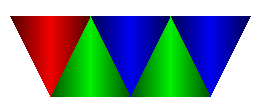
\includegraphics[width=0.33in]{vmw_logo.png} Production\\
by Vince `deater' Weaver, 2023
\end{center}

\pagebreak
\color{black}
\pagestyle{fancy}
\setcounter{page}{1}

\mbox{}
\vfill
\noindent
NOTE: Always turn the console {\bf POWER} switch {\bf OFF} when inserting
or removing an ATARI Game Program\textsuperscript{TM} cartridge.
This will protect the electronic components and prolong 
the life of your ATARI 2600\textsuperscript{TM} Video Computer
System\textsuperscript{TM} game.

\pagebreak

\section*{Prolog}
	A desperate man fleeing a dangerous situation falls
	in a starry void.  He escapes by touching a magical
	``linking'' book that transports him away.  The book
	continues falling and the man worries who might find it.
\vfill

\pagebreak

\section*{Story}
	You are the one who found the book!  Throwing caution
	to the wind you touch the book and end up on Myst island.

	On this island two brothers appear trapped inside books
	of their own.  They are a bit evasive about how they
	ended up in this situation.  The somewhat conniving
	brother asks you to find red pages and put then in his book.
	The somewhat unstable brother begs you to find blue pages
	and put them in *his* book.

	You solve puzzles and travel to four different fantastic worlds
	(unfortunately you cannot visit them with this cartridge
	due to size limitations).
	You bring back red and blue pages and put them in the brothers' books.
	They both want to be freed.  Who do you trust?

	While exploring you also found a torn note.
	When put together it
	looks like what is found on the following page\dots
\vfill

\pagebreak
\begin{small}
\begin{verbatim}
         MARKER SWIT /  CH VAULT ACCESS
                    |
               ISL  |  AND OF MYST
                    \
   THE VAULT IS LOC  \  ATED IN VERY PLAIN VIEW ON
     THE ISLAND OF M  |  YST AND ACCESS CAN BE
      ACHIEVED VERY  /  EASILY IF THE SIMPLE
 INSTRUCTIONS ARE   /  FOLLOWED.  FIRST, LOCATE
EACH OF THE MARKER  \  SWITCHES ON THE ISLAND.
 TURN EVERY ONE OF T \  HESE SWITCHES TO THE
 "ON" POSITION.  TH  /  EN GO TO THE DOCK AND,
AS A FINAL STEP, TU  \  RN THE MARKER SWITCH
        THERE TO TH  /  E "OFF" POSITION.
\end{verbatim}
\end{small}

	%This should be enough to finish your adventure!

\pagebreak

\section*{Directions}

\begin{list1}
\item Use the joystick to move the pointer
\item The pointer will change to indicate if you can move forward, left, right, or
	if an action is available
\item Click the button to move or do an action
\item If you appear stuck, carefully investigate the screen to see if there
	are action areas
\item The Color/BW switch lengthens scene transitions which
	might be easier on the eyes
\end{list1}

\begin{center}
{\bf Good Luck!}
\end{center}

\pagebreak

\section*{Hints / Spoilers!}

\noindent
Only read the rest of the manual if you are stuck and need help!
\vfill

\pagebreak

\begin{list1}
	\item What do I do first?
	\begin{list2}
		\item {\em Explore}
		\item {\em  Then maybe see the ripped note on page 5
			and do what it says}
	\end{list2}
	\item How many marker switches are there?
	\begin{list2}
		\item {\em There are 8}
	\end{list2}

	\item What's a marker switch?
	\begin{list2}
		\item {\em A brown box with a blue and yellow switch on top}
	\end{list2}
\pagebreak
	\item How do I turn these switches ``on''?
	\begin{list2}
		\item {\em Click on them.  When the blue handle is down
			it is on, when up it is off}
	\end{list2}

	\item Do I need to do the clock puzzle to get to one of the marker
		switches?
	\begin{list2}
		\item {\em Yes}
	\end{list2}

	\item How do I activate the clock puzzle?
	\begin{list2}
		\item {\em Click on the controls to the left
		partially obscured by the tree}
	\end{list2}

\pagebreak

	\item How do I solve the clock puzzle?
	\begin{list2}
		\item {\em There is a hint in the library}
	\end{list2}

	\item How do I find the hint in the library?
	\begin{list2}
		\item {\em Try poking things}
		\item {\em What do the picture frames do? Look around after
			poking them}
		\item {\em Note the blue frame does nothing in this version,
			in the real game you had to adjust this to get the
			proper hint}
		\item {\em You'll need to go behind the bookshelf and take the
		elevator}
		\item {\em Press the blue button to activate the elevator}
	\end{list2}

	\item I am stuck in the library!
		\begin{list2}
		\item {\em When the bookshelf opens, the front door closes\dots}
		\item {\em See if you can close the bookshelf again}
		\end{list2}

	\item I entered the time on the clock but nothing happened and now
		it won't let me leave!
		\begin{list2}
		\item {\em You have to press the red button}
		\end{list2}
\pagebreak
	\item How do I find the white page?
		\begin{list2}
		\item {\em This is a good time to re-read the torn note on page 5}
		\end{list2}

	\item I have the white page, now what?
		\begin{list2}
		\item {\em Have you tried putting the colored pages 
			into the books?}
		\item {\em Have you then looked into the books?}
		\end{list2}

	\item What does ``158'' mean?
		\begin{list2}
		\item {\em Have you fully explored the library?}
		\item {\em What about the bookshelf?}
		\end{list2}

	\item What do I do with the weird grid pattern?
		\begin{list2}
		\item {\em Have you tried going into the green fireplace?}
		\item {\em Enter the pattern and press the button on the left
			to activate}
		\end{list2}

	\item What's with the green book?
		\begin{list2}
		\item {\em Someone inside seems to be asking for a white page}
		\item {\em Maybe find a white page before going to see him}
		\end{list2}
\pagebreak
	\item I don't understand the ending!
		\begin{list2}
		\item Welcome to the club, 1993 edition.
		\item If you are trapped in a red or blue book, you shouldn't
			have trusted that brother.
		\item If you are trapped with the man w/o a white page,
			it's because
			the white page was ripped out of his Myst linking book
			and he can't return to Myst without it.
			So now you are stuck with him and the broken book
			and can't get back to Myst.
		\item If you got the ``good'' ending, the man went back and
			zapped the books of his no-good sons.
			(how permanent this is depends on how many of the
			sequels you've played)
			The man is busy writing into a book in an 
			attempt to save the world his wife is currently
			trapped on.
			He says you can link back to Myst and hang out there.
			Eventually in the sequel he'll send you to Riven
			to help rescue his wife.
		\end{list2}
\end{list1}

\end{document}
